\documentclass[conference]{IEEEtran}
\IEEEoverridecommandlockouts
\usepackage{cite}
\usepackage{amsmath,amssymb,amsfonts}
\usepackage{graphicx}
\usepackage{textcomp}
\usepackage{xcolor}
\usepackage{booktabs}
\usepackage{multirow}
\usepackage{url}
\usepackage{hyperref}
\hypersetup{colorlinks=true,linkcolor=blue,citecolor=blue,urlcolor=blue}

\begin{document}

\title{Evaluating Consequential Meaning Errors in Hindi Citizen Grievances:\\
A Challenge Set Analysis of COMETKiwi}

\author{%
\IEEEauthorblockN{Krishnam}
\IEEEauthorblockA{\textit{Department of AIML}\\KIET, Sikandra Rao, India}
\and
\IEEEauthorblockN{Krishna Varshney}
\IEEEauthorblockA{\textit{Department of AIML}\\KIET, Kasganj, India}
\and
\IEEEauthorblockN{Harshit}
\IEEEauthorblockA{\textit{Department of AIML}\\KIET, Ghaziabad, India}
\and
\IEEEauthorblockN{Kushagra Rashtogi}
\IEEEauthorblockA{\textit{Department of AIML}\\KIET, Siyana, India}
}

\maketitle

\begin{abstract}
Automated quality estimation (QE) models are increasingly considered for filtering and routing machine translation outputs in public-sector workflows. This paper investigates the diagnostic sensitivity of COMETKiwi (\texttt{wmt22-cometkiwi-da}) using a synthetic, category-balanced challenge set of 100 Hindi citizen grievance pairs spanning 10 administrative error categories. COMETKiwi demonstrates a pairwise ranking agreement of \textbf{95.00\%} (95/100) with the intended construction labels, with a mean score difference of $+0.041884$ (median: $+0.016785$). Category-level analysis reveals that high-contrast semantic errors exhibit wide score separations ($\Delta > +0.045$), while fine-grained temporal, spatial, and numeric corruptions show narrow margins ($\Delta < +0.013$). Five ranking failures are observed. This is an exploratory diagnostic study on structurally audited synthetic templates; independent bilingual human validation was not performed. These findings suggest that relying solely on aggregate QE scores in civic administrative pipelines may entail risks of failing to detect localized, consequential translation errors.
\end{abstract}

\begin{IEEEkeywords}
quality estimation, COMETKiwi, Hindi, citizen grievances, challenge set,
machine translation evaluation, administrative NLP, Indic languages
\end{IEEEkeywords}

\section{Introduction}
Public administrative systems in linguistically diverse environments increasingly
explore machine translation~(MT) to process citizen grievances in Hindi and
regional languages. Localized semantic errors---inverted service status, shifted
dates, transposed amounts, misdirected departments---can carry operational risks
in public-sector pipelines. We investigate whether \textbf{COMETKiwi}
\cite{rei-etal-2022-cometkiwi} reliably penalizes these error types.

\textbf{Research questions:}
\begin{itemize}
  \item \textbf{RQ1} (Pairwise Ranking Agreement): What is COMETKiwi's pairwise
        agreement when comparing faithful vs.\ corrupted Hindi grievance translations?
  \item \textbf{RQ2} (Category Heterogeneity): How does metric sensitivity vary
        across 10 administrative error categories?
  \item \textbf{RQ3} (Failure Morphology): In which cases does COMETKiwi rank the
        corrupted translation higher, and how often do margins fall below~0.005?
\end{itemize}

\section{Related Work}
\textbf{COMET}~\cite{rei-etal-2020-comet} demonstrated that fine-tuning cross-lingual
encoders on human Direct Assessment annotations improves MT evaluation.
\textbf{COMETKiwi}~\cite{rei-etal-2022-cometkiwi} established a leading reference-free
architecture, winning WMT22. \textbf{xCOMET}~\cite{guerreiro-etal-2024-xcomet} adds
span-level error detection. The WMT Critical Error Detection tasks
\cite{specia-etal-2020-findings,specia-etal-2021-findings,zerva-etal-2022-findings}
focus on high-resource pairs; South Asian administrative text remains less explored.
The challenge-set paradigm~\cite{isabelle-etal-2017-challenge,sennrich-2017-grammatical}
isolates specific linguistic phenomena through minimally perturbed pairs.
\textbf{IndicTrans}~\cite{ramesh-etal-2022-indictrans} and
surveys~\cite{haddow-etal-2022-survey} advance Indic MT, but domain-specific QE
evaluation on Hindi grievances remains limited.

\section{Dataset Construction}

\subsection{Error Taxonomy}
We formalize 10 administrative error categories: (1)~\textit{negation\_service\_status},
(2)~\textit{date}, (3)~\textit{duration}, (4)~\textit{amount}, (5)~\textit{location},
(6)~\textit{location\_detail}, (7)~\textit{requested\_action},
(8)~\textit{department\_routing\_correctness}, (9)~\textit{time\_reference},
(10)~\textit{urgency}.

\subsection{Compilation and Audit}
100 English--Hindi pairs (\texttt{SYN001\_hi}--\texttt{SYN100\_hi},
SHA-256: \texttt{ae04ccf2\ldots}) were consolidated from six synthetic batches.
Structural checks confirm: 100 unique pairs, 10 per category, no empty fields,
distinct faithful/corrupted texts for every pair.

\subsection{Scientific Boundaries}
The dataset is \textbf{synthetic}. Semantic labels reflect intended construction
designs. \textbf{Independent bilingual human validation was not performed.}

\section{Experimental Setup}
\textbf{Model:} \texttt{Unbabel/wmt22-cometkiwi-da} (COMET~v2.2.7).
\textbf{Device:} NVIDIA GeForce RTX~3050 Laptop GPU, batch size~2,
PyTorch~2.6.0+cu126, Python~3.12.10.
Each candidate was scored against the English source;
$\Delta = \text{faithful\_score} - \text{corrupted\_score}$;
$\Delta > 0$ = correct ranking.

\section{Results}

\subsection{Overall Pairwise Ranking Agreement}
COMETKiwi achieves \textbf{95.00\%} pairwise accuracy (95/100;
Wilson 95\%~CI: [88.82\%, 97.85\%]~\cite{wilson-1927-probable};
Clopper--Pearson 95\%~CI: [88.72\%, 98.36\%]~\cite{clopper-pearson-1934-use}).
See Table~\ref{tab:overall}.

\begin{table}[h]
\caption{Overall Pairwise Evaluation Metrics}
\label{tab:overall}
\centering
\begin{tabular}{lr}
\toprule
\textbf{Metric} & \textbf{Value} \\\midrule
Total pairs & 100 \\
Candidate inferences & 200 \\
Faithful ranked higher & 95 \\
Corrupted ranked higher & 5 \\
Ties & 0 \\
Pairwise accuracy & 95.00\% \\
Mean $\Delta$ & $+0.041884$ \\
Median $\Delta$ & $+0.016785$ \\
Std.\ dev.\ $\Delta$ & $0.053249$ \\
Min $\Delta$ & $-0.006049$ \\
Max $\Delta$ & $+0.301254$ \\
Pairs with $|\Delta|{<}0.005$ & 18 \\
\bottomrule
\end{tabular}
\end{table}

\subsection{Category-Level Analysis}
Table~\ref{tab:categories} shows per-category results.
High-contrast categories achieve 100\% accuracy with wide margins;
\textit{time\_reference} records 80\% accuracy and the smallest mean margin.
See also Fig.~\ref{fig:margins}.

\begin{table}[h]
\caption{Category-Level Pairwise Results}
\label{tab:categories}
\centering
\resizebox{\columnwidth}{!}{%
\begin{tabular}{lrrc}
\toprule
\textbf{Category} & \textbf{Acc.} & \textbf{Mean $\Delta$} & \textbf{Failures}\\\midrule
negation\_service\_status & 100\% & $+0.1390$ & 0 \\
department\_routing\_correctness & 100\% & $+0.0552$ & 0 \\
urgency & 100\% & $+0.0455$ & 0 \\
location\_detail & 100\% & $+0.0123$ & 0 \\
amount & 100\% & $+0.0113$ & 0 \\
duration & 100\% & $+0.0083$ & 0 \\
requested\_action & 90\% & $+0.1113$ & 1 \\
location & 90\% & $+0.0211$ & 1 \\
date & 90\% & $+0.0098$ & 1 \\
time\_reference & 80\% & $+0.0049$ & 2 \\
\bottomrule
\end{tabular}%
}
\end{table}

\subsection{Failure Analysis}
Five inversions: SYN007 (\textit{requested\_action}, $\Delta{=}{-}0.000551$),
SYN025 (\textit{location}, $\Delta{=}{-}0.000628$),
SYN002 (\textit{date}, $\Delta{=}{-}0.001283$),
SYN079 (\textit{time\_reference}, $\Delta{=}{-}0.001592$),
SYN059 (\textit{time\_reference}, $\Delta{=}{-}0.006049$).
All occur within $|\Delta|{<}0.007$.

\begin{figure}[h]\centering
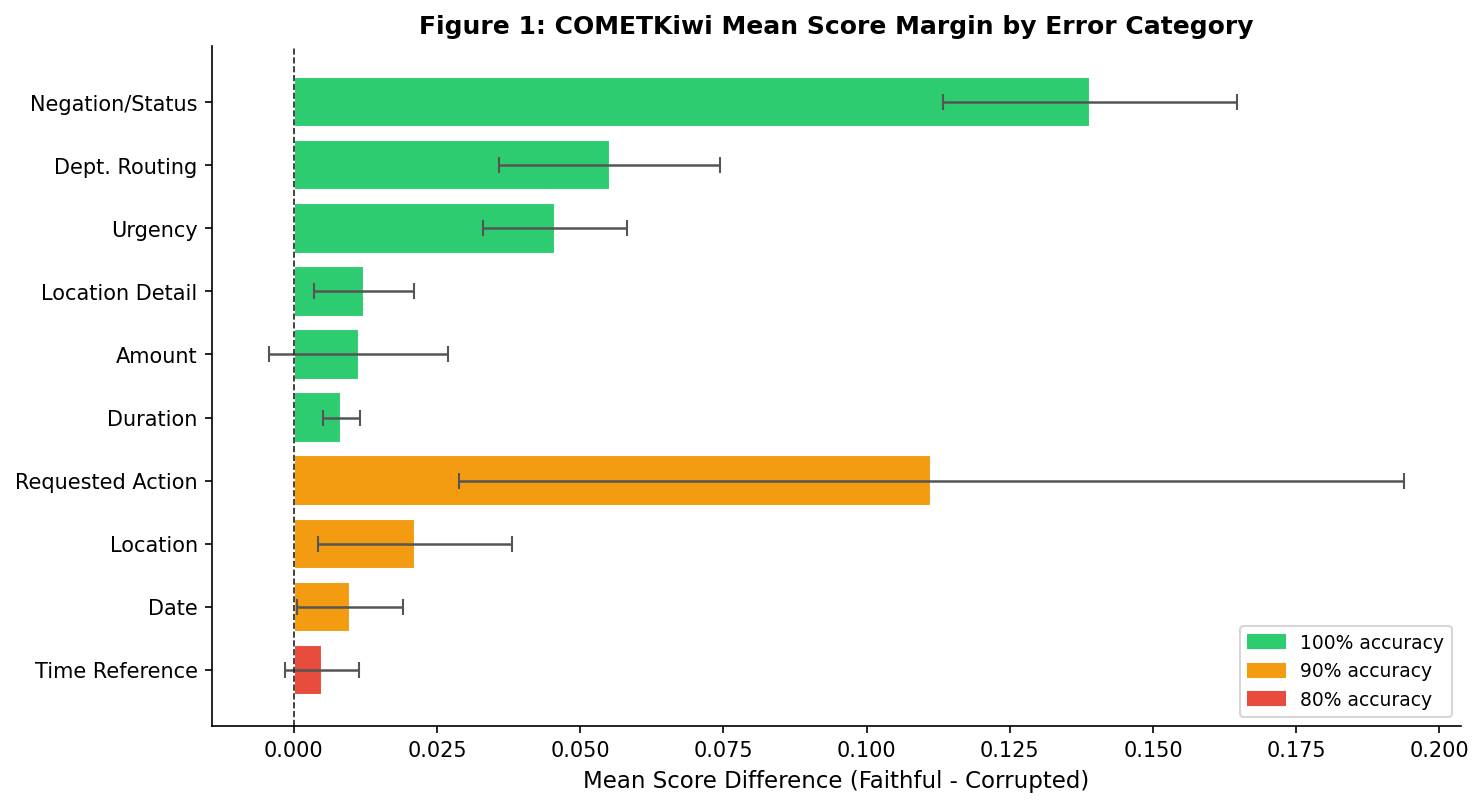
\includegraphics[width=\columnwidth]{figures/eda_category_distribution}
\caption{Mean score margin per category $\pm 1$ SD. Green = 100\%, orange = 90\%, red = 80\%.}
\label{fig:margins}
\end{figure}

\begin{figure}[h]\centering
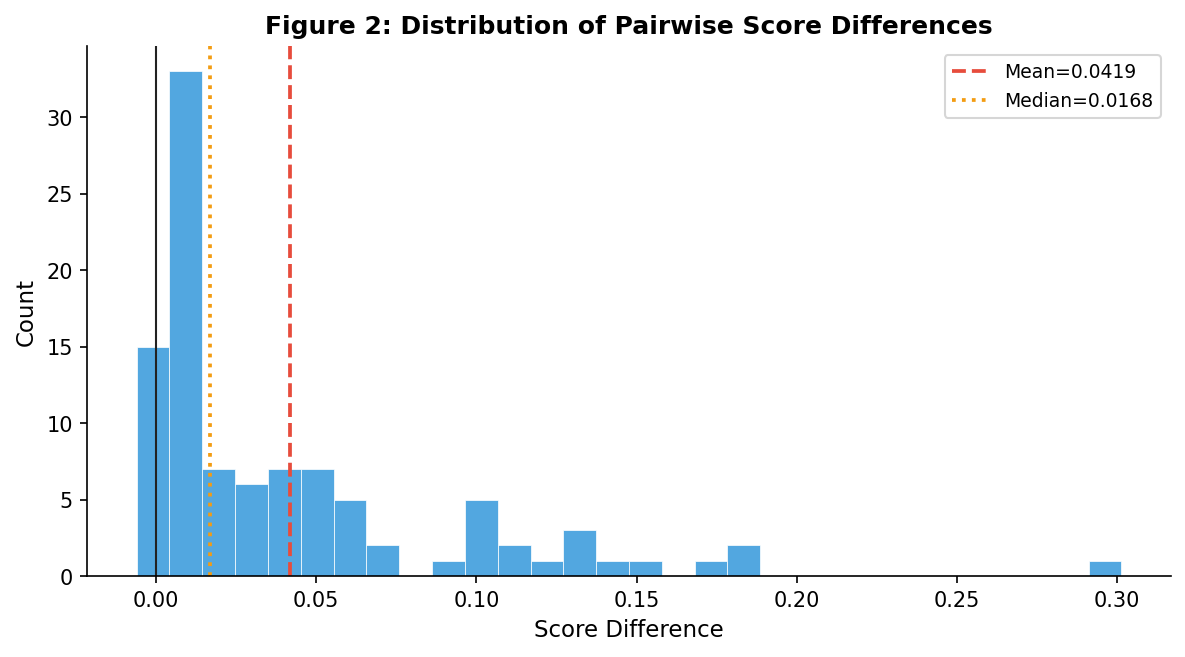
\includegraphics[width=\columnwidth]{figures/eda_score_distributions}
\caption{Histogram of pairwise score differences ($n{=}100$).}
\label{fig:hist}
\end{figure}

\begin{figure}[h]\centering
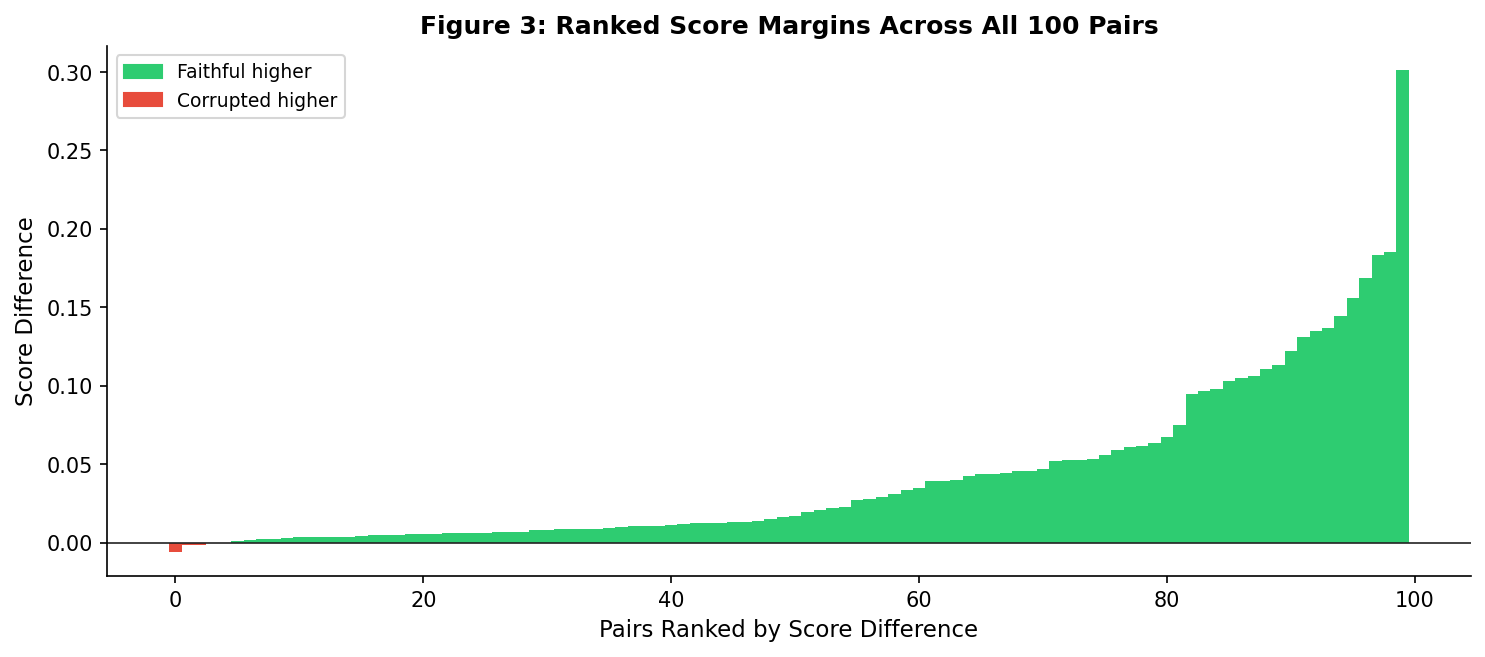
\includegraphics[width=\columnwidth]{figures/eda_score_margins_by_category}
\caption{All 100 pairs ranked by score difference; red = ranking failure.}
\label{fig:ranked}
\end{figure}

\section{Discussion and Limitations}
The 95\% aggregate accuracy is encouraging, but five inversions and 18 near-zero
margins in fine-grained categories reveal a diagnostic gap. Temporal references,
minor location substitutions, and short date shifts produce near-zero $\Delta$,
leaving COMETKiwi effectively blind to these perturbations.

\textbf{Limitations:}
(1)~\textit{Synthetic data}---results may not generalize to natural grievances.
(2)~\textit{No independent human validation}---95\% is relative to intended
construction labels only.
(3)~\textit{Single model, single language pair}---findings specific to
\texttt{wmt22-cometkiwi-da} and English--Hindi.
(4)~\textit{No demonstrated real-world harm} from any production MT system.

\section{Conclusion}
This exploratory diagnostic analysis shows COMETKiwi achieves 95\% pairwise
accuracy on a 100-pair synthetic Hindi grievance challenge set, but is not
reliably sensitive to fine-grained temporal, spatial, and numeric corruptions.
These findings motivate future work on domain-specific QE evaluation, independent
bilingual human validation, and Indic administrative challenge-set construction.

\bibliographystyle{IEEEtran}
\bibliography{references}

\end{document}
